\documentclass[12pt, titlepage]{article}
\usepackage{float}
\usepackage{graphicx}
\usepackage{booktabs}
\usepackage{tabularx}
\usepackage{hyperref}
\usepackage{hhline}
\usepackage{extsizes}

\hypersetup{
    colorlinks,
    citecolor=black,
    filecolor=black,
    linkcolor=red,
    urlcolor=blue
}
\usepackage[round]{natbib}

\title{SE 3XA3: Test Plan\\ ChessAce}

\author{Team 18, Team MIF
		\\ Jerry Ke, kex1
		\\ Harry fu, fuh6
		\\ Morgan Cui, cuim2
}

\date{\today}

\begin{document}

\maketitle ~\cite{SRS}

\pagenumbering{roman}
\tableofcontents
\listoftables
\listoffigures

\begin{table}[bp]
\begin{tabularx}{\textwidth}{p{3cm}p{2cm}X}
\toprule {\bf Date} & {\bf Version} & {\bf Notes}\\
\midrule
2018-10-7 & 1.0 & Draft and Template\\
2018-10-26& 1.1 & All section completed\\
\bottomrule
\end{tabularx}
\caption{\bf Revision History}
\end{table}

\newpage

\pagenumbering{arabic}

\section{General Information}

\subsection{Purpose}
The purpose of this test plan is to build the confidence that the software for the project is implemented correctly. Also, it provides evidence and record for future investgation.

\subsection{Scope}
The Test Plan presents a guideline for testing the functionality of the re-implementation of ChessOOP project. The objective of this Test plan is to verify that the re-implementation has met the the requirements specified in the SRS document, and construct methods to make completion of requirement be measurable and quantifiable. \\
The Test Plan will record what is to be tested of the software, and what testing methods and tools the test team will be using.


\subsection{Acronyms, Abbreviations, and Symbols}
\begin{table}[!htbp]
	\centering
	\begin{tabular}[pos]{|l|l|}
		
		\hline
		\textbf{Term}& \textbf{Definition} \\ \hline
		PoC & Proof of Concept \\ \hline
		SRS & Software Requirements Specification \\ \hline
		GUI & Graphical User Interface \\ \hline
	\end{tabular}
		\caption{\bf Table of Abbreviations}
	\label{table1}
	\end{table}

\begin{table}[H]

	\begin{tabular}[pos]{|l|l|}
		\hline
		%\label
		\textbf{Term}& \textbf{Definition} \\ \hline
		Structural Testing & Testing derived from the internal structure of the software. \\ \hline
		Functional Testing & Testing derived from a description of how the program functions.  \\ \hline 
		Dynamic Testing & Testing which includes having test cases run during execution. \\ \hline
		Static Testing & Testing that does not involve program execution.  \\ \hline  
		Manual Testing & Testing conducted by people. \\ \hline
		Automated Testing & Testing that is run automatically by software. \\ \hline 
	\end{tabular}
		\caption{\bf Table of Definitions}
		\label{table2}
\end{table}	


\subsection{Overview of Document}
The ChessAce project will re-implement the open source project ChessOOP. By using the same programming language, ChessAce will retain all requirements, and perfect the missing concepts from ChessOOP.  All software's requirements are numbered in the SRS document.
\section{Plan}
	
\subsection{Software Description}
The software will allow users to play Chess game against oneself or other human players on the same machine. The implementation will be completed in Java.

\subsection{Test Team}
Team MIF is responsible for testing this software. The members of Team MIF are Morgan Cui, Harry Fu, Xingjian Ke

\subsection{Automated Testing Approach}
Test automation of ChessAce will be perform unit test via Junit tool comes with Eclipse IDE. Junit test files will be implemented based on consideration of boundary cases for different pieces, including cases about movement, elimination, transfomation, stalemate, and other special operations. Above boundary cases will be tested on a designed board state to imitate some extreme cases. Such tests will be automatically executed before every commit to ensure the correctness of implementation.

\subsection{Testing Tools}
The test tool for this software will be Junit. It will be used to automate the unit testing. Also, EclEmma, which is a built-in function for Eclipse Photon, will be used for code coverage check.
\begin{figure}[h]
  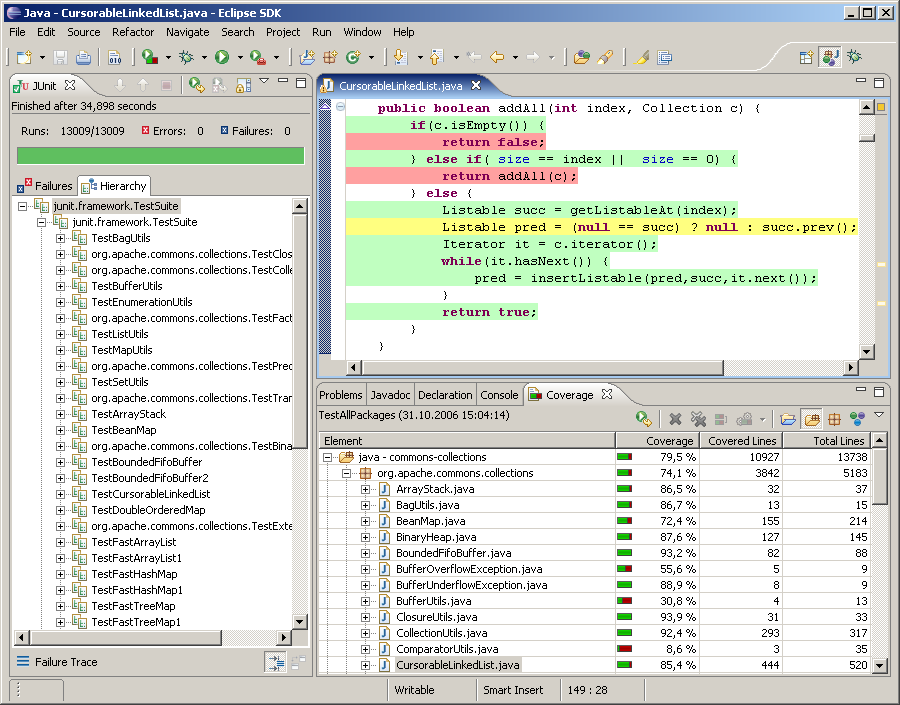
\includegraphics[width=\linewidth]{screen.png}
  \caption{Sample of EclEmma}
  \label{fig:Ecl}
\end{figure}~\cite{EclEmma}

\subsection{Testing Schedule}

\begin{figure}[H]
  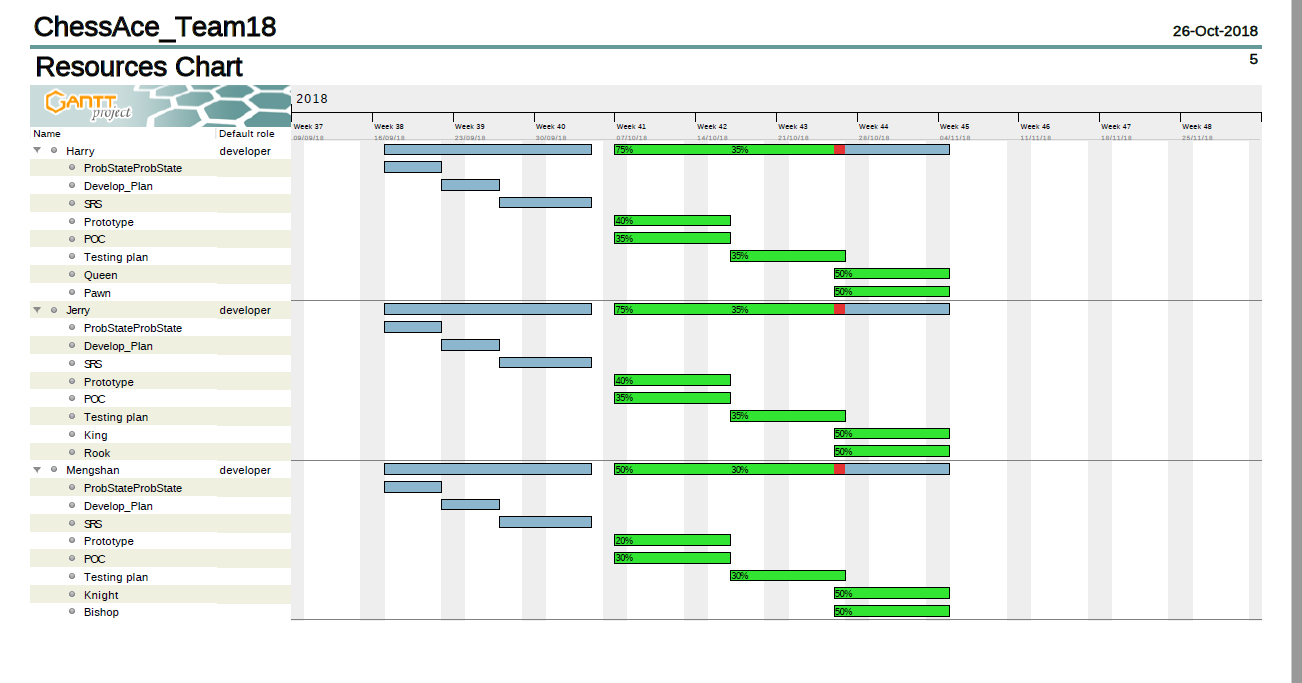
\includegraphics[width=\linewidth]{schedule.png}
  \caption{Gantt Schedule}
  \label{fig:schl}
\end{figure}

For more detailed information, please see the attached gan project and pdf in the local path.
\section{System Test Description}
	
\subsection{Tests for Functional Requirements}

\subsubsection{User Input}
		
\paragraph{Mouse click testing}

\begin{enumerate}

\item{FT-MSC-1\\}

Type: Functional, Dynamic, Manual
					
Initial State: Chess game is currently in progress
					
Input/Condition: User clicks on a piece and then clicks another cell.
					
Output/Result: Piece move to an empty cell or eliminate oppsite's piece or can't do movement if there exists a same color piece
					
How test will be performed: The program will be run given the specific inputs. Following that we will check to make sure that the response was correct. Whether it move as we expect or does not move any more. 
					
\item{FT-MSC-2\\}

Type: Functional, Dynamic, Manual
					
Initial State: Chess game is currently in progress
					
Input: User clicks on a piece
					
Output: All the possible move cells will be highlighted
					
How test will be performed: The program will be run given the specific inputs. Following that we will check to make sure that the response was correct. Whether if there any cell been highlighted and all the possible move cells are correct or it will not happen.

\item{FT-MSC-3\\}

Type: Functional, Dynamic, Manual
					
Initial State: Chess game is currently in progress
					
Input: User clicks on a piece and then click on another pieces 
					
Output: The previous piece would be unselected and the current piece would be selected. 
					
How test will be performed: The program will be run given the specific inputs. Following that we will check to make sure that the response was correct. Whether if one piece is unselected and the ohter is selected.

\item{FT-MSC-4\\}

Type: Functional, Dynamic, Manual
					
Initial State: Chess game is currently in progress
					
Input: User clicks on the undo button
					
Output: The chess board go back to the state which one movement before
					
How test will be performed: The program will be run given the specific inputs. Following that we will check to make sure that the response was correct. Whether if the board went back or not.

\end{enumerate}

\subsubsection{Algorithm}

\begin{enumerate}

\item{FT-ALG-1\\}

Type: Functional, Dynamic, Manual
					
Initial State: Chess game is currently in progress
					
Input/Condition: There is no possible move for all pieces in one side
					
Output/Result: The program should return checkmate 
					
How test will be performed: The chess game will in progress and the links tested to make sure that the program could show checkmate 
					
\item{FT-ALG-2\\}

Type: Functional, Dynamic, Manual
					
Initial State: Chess game is currently in progress
					
Input: User clicks undo button twice in one turn
					
Output: The system will not allow user to do undo request twice per turn
					
How test will be performed: The program will be run given the specific inputs. Following that we will check to make sure that the response was correct. 

\end{enumerate}

\subsubsection{Graphical user interface}

\begin{enumerate}

\item{FT-GUI-1\\}

Type: Functional, Dynamic, Manual
					
Initial State: Chess game is currently in progress
					
Input/Condition: User clicked start game
					
Output/Result: There will be a timer showed on the main screen
					
How test will be performed: The chess game will in progress and the links tested to make sure there is a timer appeared on the main screen. 

\item{FT-GUI-2\\}

Type: Functional, Dynamic, Manual
					
Initial State: Chess game is currently in progress
					
Input: User clicked start game and finished move pieces
					
Output: The current player will be showed on the screen and will be changed after players moved pieces
					
How test will be performed: The chess game will in progress and the links tested to make sure the main screen shows current player and is changed each turn

\item{FT-GUI-3\\}

Type: Functional, Dynamic, Manual
					
Initial State: Chess game is currently in progress
					
Input: User select to forfeiting the game
					
Output: The program will show a confirm dialog to user
					
How test will be performed: The chess game will in progress and the links tested to make sure the main screen shows a confirm dialog before forfeiting

\end{enumerate}

\subsubsection{data storage}

\begin{enumerate}

\item{FT-DS-1\\}

Type: Functional, Dynamic, Manual
					
Initial State: Before starting game
					
Input/Condition: Two prople select to become white player and black player to play this game
					
Output/Result: This game will store the players' state and sign them to different player type
					
How test will be performed: The chess game will in progress and the links tested to make sure the game could store information of two players

\item{FT-DS-2\\}

Type: Functional, Dynamic, Manual
					
Initial State: Main screen
					
Input: The player select start game
					
Output: The white player could move first
					
How test will be performed: The chess game will in progress and the links tested to make sure the white player could move piece first

\item{FT-DS-3\\}

Type: Functional, Dynamic, Manual
					
Initial State:  Chess game is currently in progress
					
Input: User clicked start game and finished move pieces
					
Output: The program can save the latest record of the game
					
How test will be performed: The chess game will in progress and the links tested to make sure the program could save the latest record

\end{enumerate}

\subsection{Tests for Nonfunctional Requirements}

\subsubsection{Usability}

\begin{enumerate}

\item{NF-1\\}

Type: Functional, Dynamic, Manual

Initial State: program downloaded from GitLab website onto system but not launched

Input/Condition: launch program on computers whether the operating system is Windows, Mac OS or Linux.

Output/Result: program should launch successfully and output a setup menu

How Test Will Be Performed: Program will be downloaded onto computers and the program will be checked on each operating system to determine if it runs successfully and able to perform its main function. This will ensure that users of these platforms can use the program.

\item{NF-2\\}

Type: Functional, Dynamic, Manual

Initial State: program downloaded onto system and newly launched without input provided to system

Input/Condition: users are asked to setup, choosing the role of a chess game and setting the timer 

Output/Result: after the two roles were chosen and the timer is set, the game starts. Most of users can successfully start the game without assistance within 2 minutes

How Test Will Be Performed: a test group of people whose age is above 6 and know how to use computers are asked to start the game using this program, which is launched for them. The time it takes for them to determine how to use the program and successfully perform the requested action by producing a chess game board. The majority of the test group must have produced a recording within 2 minutes for this test to be considered successful.

\item{NF-3\\}

Type: Functional, Dynamic, Manual

Initial State: users in test group have already performed the preceding two tests by downloading the program to their computer and display a standard 8 * 8 chess board on the screen using the program

Input/Condition: users in test group are asked to rate the program on the criteria of ease of download, ease of use, understandability of text and symbols, and overall satisfaction on a scale from 1 to 5

Output/Result: the average rating from the test group on all categories is higher than 3

How Test Will Be Performed: a test group of people who has a basic idea of chess play will be provided with a questionnaire that provides a list of criteria and a scale for each where 1 represents Very Poor, 2 represents Below Expectations, 3 represents Satisfactory, 4 represents Above Expectations, and 5 represents Excellent. Test group will be asked to rate the program on the provided criteria using the given scale. The average rating for each criterion will be calculated. The average must be above 3 on each criterion.


\item{NF-4\\}

Type: Functional, Dynamic, Manual

Initial State: users in test group have already performed the preceding two tests by downloading the existing implementation of the program to their computer and displaying a chess game board on the computer screen using the existing implementation of the program

Input/Condition: users in test group are asked to rate the existing implementation of the program on the criteria of ease of download, ease of use, understandability of text and symbols, and overall satisfaction on a scale from 1 to 5

Output/Result: the average rating from the test group on each category from test SS-3 is equal to or higher than the average rating from the test group on the corresponding category in this test, SS-4.

How Test Will Be Performed: each user in the test group who has a basic idea of chess play will be provided with a questionnaire that provides a list of criteria and a scale for each where 1 represents Very Poor, 

\subsubsection{Performance}

\item{NF-5\\}

Type: Functional, Dynamic, Manual

Initial State: program is launched and on default settings, with all required settings for starting a chess game having been set

Input/Condition: chess board initiated

Output/Result: the requested action is performed in under PROCESSING-TIME which is no more than 10 seconds.

How Test Will Be Performed: either a group of users will be asked to perform the task or the task will be iterated multiple times. The time elapsed between the recording of the screen being initiated by properly set 3 options and the program actually displaying a chess board then starting a chess game will be measured. The requested action must be performed under PROCESSING-TIME for USER-TESTPERCENTAGE of the times the test is performed.

\item{NF-6\\}

Type: Functional, Dynamic, Manual

Initial State: program is launched and on default settings, in the process of playing a chess game

Input/Condition: once the time interval between two valid moves exceed the initial setting time.

Output/Result: the game ended and current player lose the game

How Test Will Be Performed: each user in the test group who has a basic idea of chess play will be asked to perform the task or the task will be iterated multiple times. When there is a over timing between two moves, the program will be ended and current player lose the game. This will ensure the program execute normally when this situation occurred.

\item{NF-7\\}

Type:  Functional, Dynamic, Manual

Initial State: users in test group have already downloaded the program to their computer and display a chess game board on the screen using this program 

Input/Condition: users in test group are asked to complete a full chess game

Output/Result: the player can only move the pieces of the pre-selected side.

How Test Will Be Performed: each user in the test group who has a basic idea of chess play users will be asked to perform the task or the task will be iterated multiple times. When the user playing the game, the move can be valid only if the piece is moved to the pre-selected side. This will ensure the correct chess game rule is provided. 

\item{NF-8\\}

Type: Functional, Dynamic, Manual

Initial State: users in test group have already downloaded the program to their computer and display a chess game board on the screen using this program 

Input/Condition: users in test group are asked to complete a full chess game

Output/Result: the selected chess piece must move to the user selected valid square.

How Test Will Be Performed: each user in the test group who has a basic idea of chess play users will be asked to perform the task or the task will be iterated multiple times. When the user playing the game, the selected chess piece should display properly to valid square. This will ensure the chess game can be executed successfully. 

\end{enumerate}

\subsection{Traceability Between Test Cases and Requirements}

\begin{figure}[H]
  \includegraphics[width=\linewidth]{trace1.png}
  \caption{Traceability Matrix 1}
  \label{fig:tra1}
\end{figure}

\begin{figure}[H]
  \includegraphics[width=\linewidth]{trace2.png}
  \caption{Traceability Matrix 2}
  \label{fig:tra2}
\end{figure}

Corresponding Excel file attached in the local path
\newpage

\section{Tests for Proof of Concept}

Proof of Concept  Test inherits from Section 3 with two additional cases

\subsection{Rules of the Game}
		
\paragraph{Movement and Transformation}

\begin{enumerate}


\item{POCT-1\\}

Type: Functional, Dynamic, Manual, Static etc.
					
Initial State: program is launched and on default settings, in the process of playing a chess game. Board state is unknown.
					
Input: users in test group are asked to perform a castling movement.
					
Output: The select king and the rook on the moving direction perform castling under valid condition. Else, board state remains the same.
					
How test will be performed:  The chess game will in progress and the links tested to make sure the king and rook can perform castling
					
\item{POCT-2\\}

Type: Functional, Dynamic, Manual, Static etc.
					
Initial State:  program is launched and on default settings, in the process of playing a chess game. Board state is unknown.
					
Input: users in test group are asked to perform a pawn to queen transformation.
					
Output: The select pawn transform to queen when it reaches the other end of the board. Else, board state remains the same.
					
How test will be performed:  The chess game will in progress and the links tested to make sure the pawn could do promotion if all the constraints are satisified. 

\end{enumerate}
\section{Comparison to Existing Implementation}
	
\begin{enumerate}
\item {NF-4 in Tests for Nonfunctional Requirements(Usability)} (Usability)

This test is designed for comparing ChessAce to existing implementation, of the program on the criteria of ease of download, ease of use, understandability of text and symbols, and overall satisfaction on a scale from 1 to 5. The average rating of ChessAce should be equal or higher than existing implementation. 

\item POC test cases are about two basic movements not included in the existing implementation.
\end{enumerate}		
\newpage
\section{Unit Testing Plan}

The Junit Framework will be used to perform unit testing for this project. EclEmma will help identify the code coverage of the test.		

\subsection{Unit testing of internal functions}
Unit test of internal functions will test any methods that return values or modify values. For any method not directly relates to the state of the chess board, unit test can be acomplished by providing a sample object, such as piece and board cell, and verify the output with expected results after the method call. Unit test will include tests that contain propar inputs and inputs that generate exceptions. This project will not import any stubs or drivers specifically for testing purposes. All necessary components will already be included in the class implementation. Unit test will use EclEmma to help identify the code coverage during the process. Our goal is to maximize function and branch converage to 100\%, and hit 80\% of statement coverage.
\subsection{Unit testing of output files}		
Since the implementation of ChessAce project results in a game with GUI, any visual output is strictly relate to some internal function call. The only testing purpose here is to determine if the mouse-click will return a unexpected coordination output. On the other hand, unit test of output files should check if mouse-click operation returns the expected result same with operating with corresponding console commands. Also, mouse clicks outside the board area should also be checked to see if such click event returns invalid output.

\newpage

\section{Appendix}



\subsection{Symbolic Parameters}


\subsection{Usability Survey Questions?}

\bibliographystyle{ieeetr} 
\bibliography{SRS} 

\end{document}